\documentclass{llncs}

\usepackage{graphicx}
\usepackage{graphics}
\usepackage{epsfig}
\usepackage{verbatim}
\usepackage{amsmath}
\usepackage{xspace}

\newcommand{\nop}[1]{}
\newcommand{\su}[1]{} %{{\em #1}}

\newcommand{\CV}{\ensuremath{\mathcal{C}_{V}}\xspace}
\newcommand{\PdtV}{\ensuremath{\mathcal{P}_{V}^{dt}}\xspace}
\newcommand{\PoV}{\ensuremath{\mathcal{P}_{V}^{o}}\xspace}
\newcommand{\PV}{\ensuremath{\mathcal{P}_{V}}\xspace}
\newcommand{\XV}{\ensuremath{\mathcal{X}_{V}}\xspace}

\newcommand{\CRDF}{\ensuremath{\mathcal{C}_{RDF}}\xspace}
\newcommand{\PRDF}{\ensuremath{\mathcal{P}_{RDF}}\xspace}
\newcommand{\PdtRDF}{\ensuremath{\mathcal{P}_{RDF}^{dt}}\xspace}
\newcommand{\PoRDF}{\ensuremath{\mathcal{P}_{RDF}^{o}}\xspace}
\newcommand{\XRDF}{\ensuremath{\mathcal{X}_{RDF}}\xspace}

\newcommand{\CRDFS}{\ensuremath{\mathcal{C}_{RDFS}}\xspace}
\newcommand{\PRDFS}{\ensuremath{\mathcal{P}_{RDFS}}\xspace}
\newcommand{\PdtRDFS}{\ensuremath{\mathcal{P}_{RDFS}^{dt}}\xspace}
\newcommand{\PoRDFS}{\ensuremath{\mathcal{P}_{RDFS}^{o}}\xspace}
\newcommand{\XRDFS}{\ensuremath{\mathcal{X}_{RDFS}}\xspace}

\newcommand{\COWL}{\ensuremath{\mathcal{C}_{OWL}}\xspace}
\newcommand{\POWL}{\ensuremath{\mathcal{P}_{OWL}}\xspace}
\newcommand{\PdtOWL}{\ensuremath{\mathcal{P}_{OWL}^{dt}}\xspace}
\newcommand{\PoOWL}{\ensuremath{\mathcal{P}_{OWL}^{o}}\xspace}
\newcommand{\XOWL}{\ensuremath{\mathcal{X}_{OWL}}\xspace}


\begin{document}

\title{Weaving the Pedantic Web\thanks{This work has been supported by Science Foundation Ireland (SFI/02/CE1/I131).}}

\titlerunning{Weaving the Pedantic Web}

\author {Team Alpha}

%
\authorrunning{Team Alpha}   % abbreviated author list (for running head)
%
%%%% modified list of authors for the TOC (add the affiliations)
\institute{National University of Ireland, Galway \\
Digital Enterprise Research Institute\\
\email{firstname.lastname@deri.org}}


% typeset the title of the contribution

% CONVENTIONS FOR USE...
% English-UK.
% Capitalise 'the Web' and 'the Semantic Web' when used as a noun, not when used as an adjective 'web data', 'semantic web data'
% 'Data' is plural: the data reside within documents, the data are chaotic...


\maketitle

\begin{abstract}
In this paper we provide detailed discussion regarding common mistakes and issues relating to publishing RDF data on the Web.
In particular, we discuss the cause and possible solutions to the highlighted issues; we categorise the highlighted problems according to their severity and possible knock-on side effects.
Throughout, we provide statistics and examples from the Web to highlight the prevalence and severity of various observed anomalies in RDF web data.
Continuing, we present and evaluate a system which can be used by publishers to validate their RDF data with respect to our commonly observed mistakes.
\end{abstract}

%\newpage

%\tableofcontents

%\newpage

%############################################################################################
\section{Introduction}\label{sec:intro}
%############################################################################################

There has been continuous growth in both the scale and diversity of data published to the Web.
The Semantic Web movement aims to bring order to this data by providing a stack of technologies, the core of which is the Resource Description Framework (RDF) for publishing data in a machine-readable format: there now exists millions of RDF data-sources on the Web contributing billions of statements.
The Semantic Web technology stack includes means to supplement instance data being published in RDF with ontologies described in RDF Schema (RDFS)~\cite{key:rdfschema} and the Web Ontology Language (OWL)~\cite{key:owl}, allowing people to formally specify a domain of discourse, and providing machines a more sapient understanding of the data.
In particular, the enhancement of instance data with structural data published in ontologies allows for reasoning.

However, such an advancement in knowledge representation on the Web has inevitabily lead to many teething problems relating to how and where RDF data is published, what is being said, how the data is represented in RDF, how described resources should be identified and, perhaps most problematically, whether or not the document and it's surrounding ontologies are consistant according to reasoning.
These problems are not only present in low-volume publishing, such as the manual crafting of single RDF documents, but are also worringly present in high-volume publishing, such as various RDF exporter systems.

With regards RDF, there is no clear way of validating that the document is correctly published and that the data is represented correctly.
Oftentimes, a publisher will have to rely upon their experience and know-how with varying success.
Errors may arise from a protocol and syntax level, mis-identification (or lack of identification) for resources described, non-authoritative assertions in ontologies, inconsistancies revealed by reasoning and use of unreachable, undefined or deprecated ontology concepts.
These errors have varying side-effects: e.g., documents not being retrievable, not being parsable, describing something other than intended, describing something not adequately identified, causing incomplete reasoning and causing undesirable reasoning consequences.
Indeed, errors (or purposefully malignant) constructs in RDF documents may not only affect interpretation of the local document, but also negatively affect interpretation of remote documents.

All of these issues are related in that they are symptomatic of how the machine accesses and interprets the document and relevant surrounding documents; thus, in this paper we not only identify common issues but propose a system that will attempt to access and interpret the document and it's surrounding/related documents according to a given fragment of reasoning, flag any abnormalities and present the results to it's publisher.

This work has been inspired by work within the Semantic Web Search Engine project (SWSE), which aims to provide search and querying over the loosely co-ordinated RDF knowledge base burgeoning on the Web.
Through work on crawling, reasoning and query answering over RDF data on the Web, we have been privy to the chaotic nature of RDF web data through our experiences in developing, debugging and testing an end-user system intended to operate over such data.
We have had to incorporate numerous algorithms and compromises into our components in order to be suitably tolerant to the anarchic nature of web data.
Now, by identifying common issues, we hope that publishers will be more conscious of following best-practices and avoid the common pitfalls associated with their task.
We also hope that our system will be a first step towards an improvement in the quality of RDF data published on the Web.

To summarise, in this paper we take the following steps towards redressing common short-comings in RDF publishing:
\begin{itemize}
\item identify, categorize, provide examples for and discuss the severity of numerous common issues relating to RDF web data (Section~\ref{sec:issues});
\item present a system which takes as input the location of an RDF web document, provides error-checking according to the highlighted issues and provides a debug report to the publisher (Section~\ref{sec:alerts}).
\end{itemize}

\noindent
Section~\ref{sec:related} presents related work and Section~\ref{sec:conclude} concludes.

%############################################################################################
\section{Dataset}\label{sec:data}
%############################################################################################
Throughout this paper, we will present insights into the prevalence of RDF-publishing issues using a representative web dataset.
We retrieved this dataset from the Web in April 2009 by means of a web-crawl using MultiCrawler~\cite{key:multi06}. More specifically, beginning from Tim Berners-Lee's FOAF file\footnote{\url{http://www.w3.org/People/Berners-Lee/card}}, we performed a seven-hop breadth first crawl for RDF/XML files using {\small\tt Accept: application/rdf+xml}. After each hop, we extracted all URIs from the crawled data as input for the next hop. Finally, we restricted the crawl according to pay-level-domains; we enforced a maximum of 5,000 crawled documents from each domain so as to ensure a diverse and representative web dataset covering a wide spectrum of both high- and low-volume data-publishers.

The crawl consisted of access to 149,057 URLs, and acquired 54,836 (36.8\%) valid RDF/XML documents. The crawled data contains 12,534,481 RDF statements.

%############################################################################################
\section{RDF Web Data Issues}\label{sec:issues}
%############################################################################################

In this section, we enumerate and discuss issues present in RDF data published on the Web. 
In order to do so in a structured way, in Figure \ref{fig:layercake} we introduce a simplified version of the semantic web layer cake; in particular, we omit components that have not been widely adoption on the Web: signature/encryption and proof. 
Also, we include some scope for non-XML formatted RDF by including ``Structured Formats'' on the XML level.
In this section, we discuss RDF web data issues according to their position on our layer cake, progressing from the bottom up.

\begin{figure}[!ht]
\begin{center}
\includegraphics[width=.6\textwidth]{layercake.ps}
\end{center}
\caption{\label{fig:layercake} Modified semantic web layer cake}
\end{figure}

\subsection{HTTP: Protocol}
At the bottom of the stack, we must firstly have some means of publishing RDF data on the Web conformant to standard HTTP practices as defined in RFC 2616\footnote{ftp://ftp.isi.edu/in-notes/rfc2616.txt}.
With respect to this task we identify the following most pertinent and common issues present on the Web:

\begin{enumerate}
\item document not accessable from the given URL;
\item content negotiation errors;
\item mismatch between {\tt Content-Type} entity-header field and the actual format of data returned.
\end{enumerate}

\subsubsection{Document not retrievable}
Briefly, here we mean that a document URL found through crawling or by user submission does not resolve to a web document; such an attempt will unsually result in the return of a reponse code from the HTTP {\tt\small 4xx} (client error) or {\tt\small 5xx} (server error) classes.
During our crawl, a total of 7,200 (4.8\%) documents returned a {\tt\small 4xx}/{\tt\small 5xx} response code: Table \ref{tbl:45rc} summarises the results.

\begin{table}
 \begin{footnotesize}
  \begin{center}
    \begin{tabular}{r|r|r|r|r|r|r|r|r}
    {\tt\small 404} & {\tt\small 403} & {\tt\small 500} & {\tt\small 503} & {\tt\small 401} & {\tt\small 502} & {\tt\small 400} & {\tt\small 410} & {\tt\small 423} \\\hline
       6,483 & 632 & 581 & 112 & 63 & 15 & 13 & 8 & 1\\    
    \end{tabular}
    \caption{ \label{tbl:45rc}Count of {\tt\small 4xx}/{\tt\small 5xx} reponse codes returned}
  \end{center}
 \end{footnotesize}
\end{table}

\subsubsection{Faulty content negotiation}
Although a URL has resolved to a web document, the content may not abide by the HTTP content-negotiation request issued by the dowloading agent. In our scenario, we specifically refer to non-RDF/XML content being returned for the specified accept {\tt application/rdf+xml} media type; for the moment this is the only registered media type\footnote{\url{http://www.ietf.org/rfc/rfc3870.txt}} and although unofficial media types are used for other formats (e.g., {\tt text/n3}, {\tt text/rdf+n3}, {\tt application/n3}, {\tt application/x-n3}), we exclude discussion of these.
Table~\ref{tbl:cts} presents the top five returned content types of the crawled URLs using {\small\tt Accept: application/rdf+xml}; the most commonly returned content-type is in fact {\tt\small text/html} (47\%) with {\tt\small application/rdf+xml} only second (34.6\%).

\begin{table}
 \begin{footnotesize}
  \begin{center}
    \begin{tabular}{r|r|r|r|r}
    {\tt\small text/html} & {\tt\small application/rdf+xml} & {\tt\small image/jpeg} & {\tt\small text/plain} & {\tt\small text/xml} \\\hline
       70,122 & 51,532 & 6,532 & 6,206 & 5,715 \\    
    \end{tabular}
    \caption{\label{tbl:cts}Count of content-types returned }
  \end{center}
 \end{footnotesize}
\end{table}

\subsubsection{{\tt Content-Type}/actual format mismatch}
The HTTP defined {\tt Content-Type} entity-header field is intended to encode the media type of the content served to the requesting agent. However, oftentimes these do not match. During our crawl, we found that 5,967 documents returning the {\tt\small application/rdf+xml} content-type were not valid RDF/XML documents. Of these, 5,396 (90.4\%) were documents that did not contain any content (reponse code other than {\tt\small 200}). Conversely, Table~\ref{tbl:ctsrx} lists the top five content-types returned for documents found to be valid RDF/XML; in particular, 16.9\% of valid RDF/XML documents are served with a content-type other than {\tt\small application/rdf+xml}.

\begin{table}
 \begin{footnotesize}
  \begin{center}
    \begin{tabular}{r|r|r|r|r}
    {\tt\small application/rdf+xml} & {\tt\small text/xml} & {\tt\small application/xml} & {\tt\small text/plain} & {\tt\small text/html} \\\hline
       45,565 & 5,229 & 3,221 & 535 & 202 \\    
    \end{tabular}
    \caption{\label{tbl:ctsrx}Count of content-types returned for valid RDF/XML documents.}
  \end{center}
 \end{footnotesize}
\end{table}

\subsection{XML \& Structured Data Formats: Syntax}
RDF is a framework for providing structured data that can be interpreted by a machine.
RDF itself can be thought of as an assertional langauge and as such does not directly provide a syntax or grammer for publishing assertions; thus RDF publishers must decide upon some compatible structured format to use.

At the outset of the semantic web movement, publishers opted to employ the existing XML standard to describe RDF; RDF/XML is still the most popular means of publishing RDF today wherein RDF/XML is a heavily restricted form of the more generic and flexible XML language.
However, XML is not naturally suited for specifying RDF descriptions; various idiosyncratic solutions exist to support core RDF features, and as a result, RDF/XML documents are not easily interpretable by human review and manual efforts in editing RDF/XML documents often lead to syntactic errors or poorly formed RDF.
In addition, RDF/XML has practical drawbacks relating to the expense of parsing, outputting and difficulty in recovering from an incomplete data-stream.

More recently, numerous other structured formats have been created specifically for RDF, centred around the notion of publishing triples.
These include Notation3, N-Triples and Turtle.
Unlike XML (whereby a document can be valid XML but invalid RDF) if a document is valid Notation3/N-Triples/Turtle it is also automatically valid RDF.
However, in this paper we focus on RDF/XML syntax errors.
Naturally, we cannot document here each possible transgression of a syntactic grammar so we instead highlight the following syntactic issues:

\begin{enumerate}
\item invalid XML;
\item valid XML but not valid RDF;
\item unparsable datatypes.
\end{enumerate}

\subsubsection{Invalid XML}
At the most general level, an RDF/XML document may not be parsable due to XML syntax errors. These include, for example, mismatched start and end tags, undefined entities, invalid escaping of characters, encoding issues, etc. Of the 46,136 documents which return reponse code {\tt\small 200} and content-type {\tt\small application/rdf+xml}, 409 were invalid XML documents.

\subsubsection{Valid XML but invalid RDF/XML}
A document may be valid XML but invalid RDF; here we highlight the most common problem whereby the XML document does not correctly represent triples as is mandated by RDF/XML syntax~\cite{key:rdfxml}.

Publishers of RDF/XML documents sometimes neglect to ensure correct subject/predicate/object nesting in their document (introduced in~\cite{key:rdfxml} as `striping'), which results in an XML document with no clearly defined triple strata. In addition to incorrect nesting of \textit{s/p/o} nodes, a document may fail to represent triples due to mis-use of RDF syntactic shortcuts.

For the purposes of RDF/XML, there is a set of nine RDF names \{{\tt RDF}, {\tt Description},  {\tt ID}, {\tt about}, {\tt parseType}, {\tt resource}, {\tt li}, {\tt nodeID}, {\tt datatype}\} which characterise how triples should be parsed from an RDF/XML document or offer shortcuts for more succinct triple representation -- these names do not appear in the resulting RDF graph. 

Of the 46,136 documents which return reponse code {\tt\small 200} and content-type {\tt\small application/rdf+xml}, 162 were valid XML documents but invalid RDF/XML documents.

\subsubsection{Unparsable datatypes}
The last syntactic issue we will look at in this paper is that of malformed datatype literals; here, we specifically refer to simple built-in XML Schema datatypes~\cite{key:xmlsdts} as opposed to user-defined datatypes or enumerated datatypes. Errors occur when a datatype literal is defined which is outside of the lexical space of that datatype, and thus the value of the literal cannot be interpreted by a datatype-aware agent.

...

\subsection{RDF: Conformance}
Once a document has been successfully retrieved and parsed into triples, there may still exist issues on RDF level. 
There is a set of URI names which are reserved by the RDF specification for special interpretation in a set of triples; although the RDF specification does not formally restrict usage of these reserved names, misuse is often not deliberate and can cause unwanted consequences further up the semantic web layer cake.
Thus, although the following issues cannot be considered erroneous within the RDF layer itself, they originate from this layer and surface further up the stack; we introduce them now:

\begin{enumerate}
\item branching, cyclic or non-terminated collection lists
\item misuse of container vocabulary
\item poorly formed reification constructs
\end{enumerate}


\subsubsection{Atypical collection usage}
Although not formally disallowed by the RDF specification, atypical collection usage is often unintended and can cause unwanted consequences. Here we are concerned with the RDF collection vocabulary which consists of four constructs: \{{\tt List}, {\tt first}, {\tt rest}, {\tt nil}\}. 

Most commonly collections are not correctly terminated by the {\tt rdf:nil} construct; however, branching and cyclical lists are also evident on the Web.

...statistics

\subsubsection{Atypical container usage}
A related issue is that of atypical container usage, which is concerned with atypical usage of the following four constructs: \{{\tt Bag}, {\tt Seq}, {\tt Alt}, {\tt \_1...\_n}\}.

...

\subsection{RDFS/OWL: Compliance and Versioning}
\begin{enumerate}
\item non-standard use of RDFS/OWL
\item non-abidance to OWL abstract syntax
\end{enumerate}

\subsubsection{Non-standard RDF(S)/OWL usage}
Although not restricted by the RDF specification, the semantics and specifications of the core RDF vocabularies suggests a conventional usage of core RDF(S)/OWL terms.
Usage of a vocabulary outside of its conventionally understood semantics is termed ``non-standard use''~\cite{Bruijn-Heymans-LogiFoun-07,muno-etal-2007}.
Here, we define non-standard usage as follows:

\begin{definition} \label{def:tbox}
A triple $t$ has \emph{non-standard vocabulary usage} with respect to vocabulary V = ($\PV,\PoV,\PdtV,\CV,\XV$) -- where $\PV$ is the set of unrestricted properties in vocabulary V, $\PoV$ is the set of properties expecting a blank node/URI object (possibly typed as {\tt owl:ObjectProperty}), $\PdtV$ is the set of properties expecting a literal object (possibly typed as {\tt owl:DatatypeProperty}), $\CV$ is the set of classes and $\XV$ is the set of instances -- if one of the following conditions hold: 
\begin{enumerate}
\item a property in $\PV \cup \PoV \cup \PdtV$  appears in a position different from the predicate position;
\item a property in $\PoV$ appears in the predicate position with a literal object;
\item a property in $\PdtV$ appears in the predicate position with a non-literal object;
\item a class in $\CV$ appears in a position different from the object position 
of an \texttt{rdf:type} triple.
\item an instance in $\XV$ appears in a predicate position or the object position of an \texttt{rdf:type} triple.
\end{enumerate}
\end{definition}

For non-standard RDF usage, let $\PRDF = \{$ {\tt\small rdf:first}, {\tt\small rdf:\_1...rdf:\_n}, {\tt\small rdf:object}, {\tt\small rdf:value} $\}$, $\PoRDF = \{$ {\tt\small rdf:type}, {\tt\small rdf:rest}, {\tt\small rdf:subject}, {\tt\small rdf:predicate} $\}$, $\PoRDF = \emptyset$, $\CRDF = \{$ {\tt\small rdf:Property}, {\tt\small rdf:XMLLiteral}, {\tt\small rdf:Bag}, {\tt\small rdf:Seq}, {\tt\small rdf:Alt}, {\tt\small rdf:List}, {\tt\small rdf:Statement} $\}$  and $\XRDF = \{$ {\tt\small rdf:nil} $\}$. 
For non-standard RDFS usage, let $\PRDFS = \{$ {\tt\small rdfs:member} $\}$, $\PoRDFS = \{$ {\tt\small rdfs:domain}, {\tt\small rdfs:range}, {\tt\small rdfs:isDefinedBy}, {\tt\small rdfs:seeAlso}, {\tt\small rdfs:subPropertyOf}, {\tt\small rdfs:subClassOf} $\}$, $\PdtRDFS = \{$ {\tt\small rdfs:comment}, {\tt\small rdfs:label} $\}$, $\CRDFS = \{$ {\tt\small rdfs:Class}, {\tt\small rdfs:Resource}, {\tt\small rdfs:Literal}, {\tt\small rdfs:Datatype}, {\tt\small rdfs:Container}, {\tt\small rdfs:ContainerMembershipProperty}, {\tt\small Statement} $\}$  and $\XRDFS = \emptyset$. Finally, for non-standrad OWL usage, let $\POWL = \{$ {\tt\small owl:hasValue} $\}$, $\PoOWL = \{$ {\tt\small owl:allValuesFrom}, {\tt\small owl:backwardCompatibleWith}, {\tt\small owl:complementOf}, {\tt\small owl:disjointWith}, {\tt\small owl:distinctMembers}, {\tt\small owl:equivalentClass}, {\tt\small owl:equivalentProperty}, {\tt\small owl:hasValue}, {\tt\small owl:imports}, {\tt\small owl:incompatibleWith}, {\tt\small owl:intersectionOf}, {\tt\small owl:inverseOf}, {\tt\small owl:oneOf}, {\tt\small owl:onProperty}, {\tt\small owl:priorVersion}, {\tt\small owl:sameAs}, {\tt\small owl:someValuesFrom}, {\tt\small owl:unionOf}, {\tt\small owl:versionInfo} $\}$, $\PdtOWL = \{$ {\tt\small owl:cardinality}, {\tt\small owl:maxCardinality}, {\tt\small owl:minCardinality}  $\}$, $\COWL = \{$ {\tt\small owl:AllDifferent}, {\tt\small owl:AnnotationProperty}, {\tt\small owl:Class}, {\tt\small owl:Datatype}, {\tt\small owl:DatatypeProperty}, {\tt\small owl:DeprecatedClass}, {\tt\small owl:DeprecatedProperty}, {\tt\small owl:FunctionalProperty}, {\tt\small owl:InverseFunctionalProperty}, {\tt\small owl:Nothing}, {\tt\small owl:ObjectProperty}, {\tt\small owl:OntologyProperty}, {\tt\small owl:Restriction}, {\tt\small owl:SymmetricProperty}, {\tt\small owl:Thing}, {\tt\small owl:TransitiveProperty} $\}$   and $\XOWL = \emptyset$.


@@@it would be nice if we could find out whether there is a newer version of some ontologies used in a document (WARNING), e.g. it looks to me as if http://www.w3.org/2002/12/cal/ical is an outdated version of http://www.w3.org/2002/12/cal/icaltzd ... BTW, the latter uses a namespace which is not dereferenceable: http://www.w3.org/2002/12/cal/icalSp

\subsection{RDF/RDFS/OWL: Identity}
Apart from retrieval and parsing of semantic web documents, which we deem to be errors on the physical level, there is also a plethora of common data-level problems. The first category we analyse is related to the identification of the resources being described in an RDF document.

There has, thus far, been little agreement upon common URIs to use for equivalent resources. This is symptomatic of a lack of standardised and consistant means of creating a URI which would be against the open nature of web publishing. 
Even aside from the creation of identifiers for resources not previously described, there has been little attention paid to using centralised services to find and re-use existing identifiers for resources.
The upshot of this is a proliferation of resource descriptions not identified by URIs (blank nodes) and a lack of agreement on URIs for equivalent resources.
The lack of any authority on URI creation/re-use has lead to the following issues we will discuss in this section:

\begin{enumerate}
\item resources with no form of identification (no inverse-functional, functional or functional-cardinality properties attached);
\item poor re-use of existing URIs for equivalent resources;
\item common 'null' values for inverse-functional properties;
\item use of document URLs or existing URIs to identify new resources;
\item lack of consistant local identifiers for equivalent blank nodes;
\item duplication of identifiers for a document caused by redirects and relative URIs or blank nodes
\end{enumerate}

Resources are also commonly identified by values for properties unique to a resource.
Such properties are termed ``inverse-functional'' and are identified in OWL as the set {\tt owl:InverseFunctionalProperty}.
Values for inverse-functional properties are more easily agreed upon as a means of identity than URIs: for the most part, such values already exist as a means of identity in the real-world -- e.g., the International Standard Book Number (ISBN) values for books, Social Security Numbers for people, etc.
In particular, identification through such unique property-value pairs is paramount for resources not identified by URI as it is the only means of identifying these resources.

The FOAF ontology, which provides a specification centred around describing people and various personal attributes, has defined a number of inverse-functional properties for identifying people.
It has become quite common to not use URIs to identify people, but instead to identify them through known values for inverse-functional properties such as {\tt foaf:homepage}, {\tt foaf:mbox} (email), {\tt foaf:mbox\_sha1sum} (encoded email to prevent spamming), amongst others.

...@@@fix flow and elucidate

@@@homonyms: rss:item http://purl.org/ontology/bibo/identifier

\subsection{Linked Data: Accessibility}
From the outset of the Semantic Web movement, there has been some confusion as to the best practices regarding how and where to publish RDF to the Web, how redirects and content negotiation should be handled and the relationship between URIs used to identify resources and the URLs that they de-reference to.
Such confusion leads to behaviour, on the part of RDF publishers, which inhibits the ability of semantic web agents to locate and retrieve RDF documents, and, in particular, RDF descriptions of URI identified resources.
In an effort to improve publishing methods, the Semantic Web Deployment Working Group\footnote{\url{http://www.w3.org/2006/07/SWD/}} provides, in the form of a W3C note, a document entitled ``Best Practice Recipes for Publishing RDF Vocabularies''\footnote{\url{http://www.w3.org/TR/swbp-vocab-pub/}} which provides guidelines on the most pertinent issues: publishing location, namespace configuration, content negotiation and dereferencing URIs.
However, there are still many documents on the Web (some of which pre-date the above W3C Note) which do not abide by these best practices.

@@@linked data, http://idi.fundacionctic.org/vapour

In this section, we enumerate some issues relating to linked data best practices; i.e., physical level issues relating to retrieving RDF data related to a given URI identified resource. Along this lines, we have identified the following issues:

\begin{enumerate}
\item namespaces have protocol error (as of 1\&2 above);
\item resources not dereferenceable (dereferenced URI has error 1\&2).
\end{enumerate}

...elucidate

\subsection{Logic: Consistancy}
\begin{enumerate}
\item {\tt ?x a owl:Nothing .}
\item {\tt ?x a ?C . ?x a ?D . ?C owl:disjointWith ?D .} @@@covered by 3???
\item {\tt ?x owl:differentFrom ?y . ?x owl:sameAs ?y .}
\end{enumerate}

@@@
differentFrom + sameAs 
:AllDifferent :distinctMembers (?x1,?x2 ... ?xN) => (?x1,?x2 ... ?xN) :differentFrom (?x1,?x2 ... ?xN) .
Contrary to earlier discussion, cannot infer differentFrom statements from cardinality constraints under the Open World Assumption (on the A-Box level). Take, for example the property parents with cardinality (minCardinality) of 2 for the class Person. If I find two parents for a Person, it may be the case that two URIs are used for the parent property, each referring to the person's mother.
That said, it may be possible to infer disjointness between classes that have incompatible cardinalities for the same (or some sub) property. This is, however, quite complex: 
?c cardinality ?i . ?c onProperty ?p . ?d cardinality ?j . ?d onProperty ?p . FILTER(?i!=?j) => ?c disjointWith ?d .
?c maxCardinality ?i . ?c onProperty ?p . ?d minCardinality ?j . ?d onProperty ?p . FILTER(?i<?j) => ?c disjointWith ?d .
type +disjoint classes (some form of differentfrom reasoning can possibly be done "per document" in a bw-chainging fashion ... aidan: draft some additional rules!) 
(on form of this would need tbox reasoning that I don't bother with at the moment... need to infer all possible subClassOf relations (1sc, 2sc...), or as many as possible for rule 4dw ...  )
1sc. ?a equivalentClass ?b . => ?a subClassOf ?b . ?b subClassOf ?a .
2sc. ?a sC ?b . ?b sC ?c . => ?a sC ?c .
3co. ?a complementOf ?b . => ?a disjointWith ?b .
4dw. ?a disjointWith ?b . ?a sC ?b . => ?a sC owl:Nothing . ?b sC owl:Nothing .
(alternatively, instead of the additional T-Box reasoning with 1sc and 2sc, we just perform check reasoning on an instance of each class and flag the class if we infer ?x a owl:Nothing ).
flag triples of the type ?x sC owl:Nothing .
type owl:Nothing
datatype clashes (or are these purely syntactic... check in ter Horst paper!) 

\subsection{Trust: Authoritative Descriptions}
Within SWSE, we have developed a system for performing reasoning on the web knowledge-base consisting of crawled RDF documents: we call this system ``Scalable Authoritative OWL Reasoner'' (SAOR)~\cite{key:saoraswc}.
When initially developing the system, we quickly came to the conclusion that it is necessary to perform a restrictive form of reasoning: otherwise, we would end up with explosive inference of many non-sensical statements.
In particular, we found that for the reasoning on the Web, it was impractical to:

\begin{enumerate}
\item fully support non-standard usage of RDF;
\item allow unrestricted re-definition of classes and properties in locations independant of the authoritative spec.
\end{enumerate}



%\begin{figure}
%  \begin{center}
%    \includegraphics[width=.6\textwidth]{topical_subgraph.eps}
%  \end{center}
%  \caption{Topical subgraph for matching keyword (bold) with $n = 1, 2, 3$. Selecting larger portions of the graph before ranking yields broader results (recall up, precision down), while selecting smaller portions yields narrower results (recall down, precision up).}
%  \label{fig:topical}
%\end{figure}


%############################################################################################
\section{SWSE Alerts System}\label{sec:alerts}
%############################################################################################

%############################################################################################
\section{Related Work}\label{sec:related}
%############################################################################################

%############################################################################################
\section{Conclusion}\label{sec:conclude}
%############################################################################################

% ---- Bibliography ----
%

\bibliographystyle{abbrv}
\bibliography{paperbibtex}

\end{document} 